% ======================================================================
\section{DD size and special structures}
\label{sec:bdd_size_structures}

This section analyzes the DD size and uncovers special structures for which its size remains bounded. In what follows, we use the width of a DD $B=(N,A)$ to measure its size. Specifically, the width of layer $N_i$ for any $i \in \{1,\ldots,n\}$ is the number of nodes in such layer (i.e., $|N_i|$), and the width of $B$ is the maximum width over all layers, that is,  $\max_{i \in \{1,\ldots,n\}} |N_i|$. 

While the compact DD encoding presented in Section~\ref{sec:dds_for_bpo} gives us an extended formulation for BPO, it is exponential in size for general BPO instances, and thus, impractical. Indeed, since the DD nodes correspond to states that store subsets of hyperedges and we have at most $n = |V|$ binary variables, their width is, in the worst case, $O(2^{n-1})$. Nonetheless, we can identify structural conditions under which the DD size remains small, and, as shown in Section \ref{sec:dd_separation}, construct strong valid inequalities for these structures. In what follows, we use the set of compatible active hyperedges in a layer to characterize the size of a DD, which translates directly to DD width. We then use these results to identify hypergraph structures that can encode the BPO problem using bounded DD width and relate them to results in the literature.


\subsection{Valid antichains and compact DD width}
\label{subsec:states_valid_antichains}

We now analyze the width of the compact DD relying on the fact that active hyperedges do not behave independently. Indeed, if one hyperedge contains another, then the compatibility of the larger one forces compatibility of the other. Thus, the number of reachable states in a layer can be less than $O(2^{|E|})$ for many hypergraphs.

In what follows, we use standard terminology for posets, chains, antichains, and ideals used in discrete mathematics~\cite{stanley2012enumerative}. A \emph{poset} is a set equipped with a reflexive, antisymmetric, and transitive order. In our case, we consider set inclusions and illustrate these concepts with the poset $(2^{\{1,2,3\}}, \subseteq)$ as a running example.  A \emph{chain} is a subset of a poset in which each pair of elements is comparable, for example, $\{\{1\},\{1,2\}, \{1,2,3\}\}$ is a chain since $\{1\}\subseteq \{1,2\}\subseteq \{1,2,3\} $. An \emph{antichain} is a set of pairwise incomparable elements (e.g., $\{\{1,2\},\{2,3\}\}$). An \emph{ideal} is a downward-closed subset of a poset: whenever it contains an element, it also contains all smaller elements. Thus, if an ideal contains $\{1,2,3\}$, it must also contain every subset in the poset contained in $\{1,2,3\}$.

Now consider a DD with a vertex order $\sigma=(v_1,\ldots,v_n)$ and a layer $N_i$ for some $i \in \{1,\ldots,n\}$. For each active hyperedge $e\in\A_i$, we define its \emph{reduced active hyperedge} by $\rho_i(e)=e\cap U_i$, that is, ignoring all vertices except the ones in $U_i$. Let $\R_i=\{\rho_i(e):e\in\A_i\} $ be the set of distinct reduced active hyperedges at layer $N_i$, partially ordered by inclusion. If $R,R'\in\R_i$ are two reduced hyperedges such that  $R\subseteq R'$, then compatibility of $R'$ implies compatibility of $R$: if all assigned vertices in $R'$ have value one, then the same holds for $R$. Hence, the compatible reduced hyperedges in any reachable state form an ideal of the poset $(\R_i,\subseteq)$, and that ideal is determined by its maximal elements, which form an antichain. Note that not every antichain encodes a reachable state because the union of the antichain may force additional reduced hyperedges to be compatible. 

Given an antichain $\C$ of $(\R_i, \subseteq)$, we define
$ X(\C)=\bigcup_{R\in\C}R $ as the union of all reduced hyperedges in $\C$.
We call $\C$ a \emph{valid antichain} at layer $N_i$ if
\[
\forall R\in\R_i,\ R\subseteq X(\C)
\quad\Longrightarrow\quad
\exists M\in\C\text{ such that }R\subseteq M.
\]
In other words, an antichain is valid if every reduced hyperedge forced by setting the vertices in its union to one is already covered by one of its maximal elements. For example, if $ \{1,2\},\{2,3\},\{1,2,3\}\in\R_i$,
then $\{\{1,2\},\{2,3\}\}$ is an antichain but not a valid one, because setting elements $1,2,3$ to one also makes $\{1,2,3\}$ compatible. The valid antichain
representing that assignment is instead $\{\{1,2,3\}\}$.  Lemma \ref{lem:valid_antichains} uses these definitions and observations to characterize the reachable states at layer $N_i$ by valid antichains.

\begin{lemma}
\label{lem:valid_antichains}
Consider a vertex order $\sigma$ and a layer $N_i$ of the compact DD $B=(N,A)$. The reachable states after assigning $U_i$ variables are in bijection with the valid antichains of $(\R_i,\subseteq)$.
\end{lemma}

\begin{proof}
We first show that each reachable state in $N_i$ corresponds to a valid antichain in $(\R_i,\subseteq)$. Let $s_i$ be a reachable state and define $I(s_i)=\{\rho_i(e):e\in s_i\}\subseteq\R_i$ as the set of reduced active hyperedges that are compatible in a reachable state $s_i$. Set $I(s_i)$ is downward closed because if $R'\in I(s_i)$ and $R\in\R_i$ satisfies $R\subseteq R'$, then all vertices of $R$ also have value one under the current assignment, so $R$ is compatible as well. Therefore $R\in I(s_i)$, and $I(s_i)$ is an ideal.

Since every ideal is determined by its maximal elements, let us define
$
\operatorname{Max}(I(s_i)) = \{R\in I(s_i): \nexists R'\in I(s_i)\text{ with }R\subsetneq R'\}
$
as the set of maximal elements, which in turn form an antichain. Note that the elements in $\operatorname{Max}(I(s_i))$ are also valid: if
$R\in\R_i$ satisfies $R\subseteq X(\operatorname{Max}(I(s_i)))$, then all
vertices of $R$ have value one, so $R$ is compatible and hence belongs to $I(s_i)$. Because $I(s_i)$ is an ideal, $R$ is contained in some maximal element of $I(s_i)$.

Now, we show the other direction by assuming that $\C$ is a valid antichain. Consider the assignment on $U_i$ that sets the vertices in $X(\C)$ to one and the remaining vertices of $U_i$ to zero. Under this assignment, a reduced active hyperedge $R\in\R_i$ is
compatible if and only if $R\subseteq X(\C)$. By validity, every such $R$ is
contained in some member of $\C$. Hence, the induced state is
$
s_i(\C)=
\{e\in\A_i :
\rho_i(e)\subseteq M \text{ for some } M\in\C\}.
$
The maximal elements of the corresponding ideal are exactly the members of
$\C$. This gives the claimed bijection. \hfill$\square$
\end{proof}

Counting antichains in a general poset is \#P-complete~\cite{provanBall1983complexity},
so valid antichains are not themselves a practical algorithmic primitive. They are,
however, a useful structural guide: good orders are those that make reduced active
hyperedges comparable, or even identical, as often as possible.

We now use this notation to characterize a new family of hypergraphs that lead to polynomial-size DDs (see Theorem \ref{thm:vaw_polynomial_bdd}), and, in turn, BPO instances that can be solved in polynomial time with, for instance, the extended formulation \eqref{model:bpo-extended-dd}. To do so, let $\operatorname{VA}_i(\sigma)$ denote the set of valid antichains of
$(\R_i,\subseteq)$ at layer $N_i$ under order $\sigma$. By Lemma~\ref{lem:valid_antichains}, the compact-DD width at layer $N_{i}$ is $ |\operatorname{VA}_{i-1}(\sigma)|$. Therefore, the maximum width induced by $\sigma$ is $W(\sigma)=\max_i |\operatorname{VA}_i(\sigma)|$, and the valid-antichain width of $G$ is $\operatorname{VAW}(G)=\min_{\sigma} W(\sigma)$.

\begin{theorem}
\label{thm:vaw_polynomial_bdd}
Let $\mathcal{H}$ be a class of hypergraphs such that, for every
$G=(V,E)\in\mathcal{H}$, there exists a vertex order $\sigma$ satisfying
$W(\sigma) \le q(|V|,|E|) $
for some polynomial $q$. Then the compact DD encoding for $G$ under $\sigma$ has polynomial size. Moreover, if $q(|V|,|E|)$ is a constant, then the compact DD has $O(|V|)$ nodes and arcs.
\end{theorem}

\begin{proof}
By Lemma~\ref{lem:valid_antichains}, each layer $N_i$ contains exactly
$|\operatorname{VA}_{i-1}(\sigma)|$ reachable states, for each $i\in \{1,\ldots,n\}$ ($n = |V|$). Therefore, the number of non-terminal nodes is
\[
\sum_{i=1}^{n} |\operatorname{VA}_{i-1}(\sigma)|
\le |V|\,\max_{i\in \{0,\ldots,n-1\}} |\operatorname{VA}_i(\sigma)|  = |V|\,W(\sigma) \leq |V|\cdot  q(|V|,|E|),
\]
making the node count polynomial. Note that if $q(|V|,|E|) = q \in \mathbb{R}^+$ is a constant, the node and arc count is $O(|V|)$ because each node has at most two outgoing arcs. \hfill$\square$
\end{proof}


\subsection{Small exact DDs for literature structures}
\label{subsec:small_bdds_literature}

We now show that there exist well-known hypergraph structures with a bounded compact DD encoding. We use the previously introduced valid antichain characterization to find appropriate vertex orders that satisfy the conditions in Theorem \ref{thm:vaw_polynomial_bdd}. Specifically, we show that flowers and cycles have this property, as stated in Propositions \ref{prop:flower} and \ref{prop:cycle}, respectively. We focus on these two structures since flower~\cite{delPiaKhajavirad2018acyclic} and  $\beta$-cycle~\cite{delPiaDiGregorio2021chvatal,delPiaWalter2024simple} inequalities are based on them and are, thus, also attractive to our DD-based cutting plane approach. In what follows, a cycle hypergraph is one whose hyperedges can be ordered cyclically so that each hyperedge intersects only its two cyclic neighbors.

%The compact DD can nevertheless stay small on some of the same structures that support known BPO inequalities. The valid-antichain characterization makes this visible through appropriate vertex orders.

%We first consider cycle supports, which abstract the support structure used by $\beta$-cycle inequalities. A cycle support is a hypergraph whose hyperedges can be ordered cyclically so that each hyperedge intersects only its two cyclic neighbors. This captures the support-level structure of a $\beta$-cycle, without including the additional sign and separation conditions used by specific $\beta$-cycle inequalities~\cite{delPiaDiGregorio2021chvatal,delPiaWalter2024simple}.

\begin{proposition}\label{prop:flower}
Let $G=(V,E)$ be a flower with center hyperedge $e_0$ and petals $e_1,\ldots,e_m$. Assume the petals are pairwise disjoint outside the center and that their intersections with the center are pairwise disjoint. Then, $\operatorname{VAW}(G)\le 4$.
\end{proposition}

\begin{proof}
We first define a vertex order $\sigma$ in which the vertices in the petals are considered first, followed by the vertices at the center. Formally, consider an arbitrary petal order and, for each petal $e_j$, the order first uses the vertices
in $e_j\cap e_0$, in any order, and then the vertices in $e_j\setminus e_0$, again in any order. After all petal vertices have been ordered, order any remaining vertices of
$e_0\setminus \bigcup_{j=1}^m e_j$ arbitrarily. Because the petals are pairwise disjoint outside the center and their intersections with the center are pairwise disjoint, this order ensures that at any layer there is at most one active petal together with the center hyperedge $e_0$.

Now consider a layer in which the active petal is $e_j$. While the order is processing the vertices of $e_j\cap e_0$, every assigned vertex of $e_j$ is also an assigned vertex of the
center, so $\rho_i(e_j)\subseteq \rho_i(e_0)$. Therefore, the set of valid antichains is
$\{
\emptyset,\
\{\rho_i(e_j)\},\
\{\rho_i(e_0)\}\}
$, so there are at most three reachable states.

Then, consider a layer where we assign vertices of $e_j\setminus e_0$. The reduced petal $\rho_i(e_j)$ contains assigned vertices outside the center. In general,
$\rho_i(e_j)$ and $\rho_i(e_0)$ are then incomparable. Since no other petal is active, the set of valid antichains is
$\{\emptyset,\
\{\rho_i(e_j)\},\
\{\rho_i(e_0)\},\
\{\rho_i(e_j),\rho_i(e_0)\} \}$. Thus, there are at most four states while a petal is active. Finally, after all petals
have closed, only the center hyperedge can remain active, giving at most two reachable states. Therefore, every layer has at most four valid antichains. By Lemma~\ref{lem:valid_antichains}, the compact DD constructed from this order has width at most $4$, hence $\operatorname{VAW}(G)\le 4$. \hfill$\square$
\end{proof}

\begin{proposition}\label{prop:cycle}
Let $G=(V,E)$ be a cycle. Then, $\operatorname{VAW}(G)\le 6$.
\end{proposition}

\begin{proof}
First, we construct the vertex order in accordance with the cyclic nature of the hyperedges.  Assume that $G=(V,E)$ has $|E|= L+1$ hyperedges, choose an arbitrary hyperedge $e_0$ of the cycle, and let $e_L$ be one of its two cyclic neighbors. Let $e_1,e_2,\ldots,e_{L-1}$ be the sequence of remaining hyperedges obtained by walking around the cycle in the other direction, so that $e_{L-1}$ is adjacent to $e_L$. Then, the vertex order $\sigma$ is constructed as follows. First, consider all vertices of $e_0$ and then, for
$h=1,\ldots,L-1$, assign all not-yet-assigned vertices of $e_h$. Finally, consider the remaining vertices of $e_L$. Ties inside each hyperedge can be broken arbitrarily.

We now characterize the reachable states in each layer using valid antichains. When the vertices of $e_0$ are being assigned, the only possible active hyperedges are $e_0$ and its two neighbors, $e_L$ and $e_1$. Moreover, we have the active hyperedge relations $\rho_i(e_L)\subseteq \rho_i(e_0)$, and $\rho_i(e_1)\subseteq \rho_i(e_0)$, because every assigned vertex of $e_L$ or $e_1$ belongs to $e_0$ at this stage.  Then, the set of  possible valid antichains is $\{ 
\emptyset,\ \{\rho_i(e_L)\},\  \{\rho_i(e_1)\},\ \{\rho_i(e_L),\rho_i(e_1)\},\ \{\rho_i(e_0)\} \}$. Thus, by Lemma \ref{lem:valid_antichains}, the maximum width in these first layers is at most $5$.

Now consider a layer in which the order assigns the remaining vertices of $e_h$, with $1\le h<L-1$. At this point, only the unresolved neighbor $e_L$,
the current hyperedge $e_h$, and the next hyperedge $e_{h+1}$ may be active. Thus, the only containment relation that can arise is $\rho_i(e_{h+1})\subseteq \rho_i(e_h)$ because the only assigned vertices of $e_{h+1}$ are those already assigned inside $e_h$. Therefore, the set of possible valid antichains is $\{\emptyset,\ \{\rho_i(e_L)\},\ \{\rho_i(e_{h+1})\},\ 
\{\rho_i(e_L),\rho_i(e_{h+1})\},$ $\{\rho_i(e_h)\},\ \{\rho_i(e_L),\rho_i(e_h)\} \}$. Thus, by Lemma \ref{lem:valid_antichains}, there are at most six reachable states in such a layer.

Finally, if the current vertex corresponds to a hyperedge adjacent to $e_L$ (i.e., $e_{L-1}$), at most two reduced active hyperedges remain relevant, namely those of $e_{L-1}$
and $e_L$. If they are incomparable, the set of possible valid antichains are $\{\emptyset,\ \{\rho_i(e_L)\},\ \{\rho_i(e_{L-1})\},\ \{\rho_i(e_L),\rho_i(e_{L-1})\} \} $, and if one contains the other there are fewer. Hence, in these final layers there are at most four reachable states.

Taken together, the three cases imply that every layer has at most six valid antichains. By Lemma~\ref{lem:valid_antichains}, the compact DD constructed from this order has width at most $6$, hence $\operatorname{VAW}(G)\le 6$.
\hfill$\square$
\end{proof}

Example \ref{exa:bounded-compact-dds} illustrates the vertex order $\sigma$ defined for each hypergraph structure and the corresponding compact DD of bounded width. Also, we note that while  Proposition \ref{prop:cycle} proves that cycle hypergraphs allow a compact DD encoding of bounded size, it remains open whether $\beta$-acyclic hypergraph classes admit polynomial-size compact DDs under suitable orders. This question is distinct from the known knowledge-compilation result that bounded incidence treewidth yields a polynomial-size d-DNNF representation and polynomial-size extended formulations for BPO \cite{capelliDelPiaDiGregorio2024kc}. As shown in the following subsection, incidence-treewidth arguments do not directly carry over to our compact DD construction.


\begin{example}\label{exa:bounded-compact-dds}
Figure~\ref{fig:dd-structures} depicts the vertex orders of Propositions~\ref{prop:flower} and~\ref{prop:cycle} and the resulting bounded-width compact DDs. Figure~\ref{fig:dd-structures}(a) illustrates the two hypergraphs: on top a flower with center $e_0=\{v_1,v_3,v_5\}$ and petals $e_1=\{v_1,v_2\}$ and $e_2=\{v_3,v_4\}$, and on bottom a cycle with hyperedges $e_0=\{v_1,v_2,v_3\}$, $e_1=\{v_2,v_4\}$, $e_2=\{v_4,v_5\}$, and $e_3=\{v_3,v_5\}$. Note that vertices are numbered according to the vertex order of each DD. In both cases, the  compact DD width is bounded and slightly smaller than the worst-case scenario proved in the corresponding propositions. 
\end{example}

\begin{figure}[t]
    \centering
    \begin{minipage}[b]{0.20\linewidth}\centering
        \resizebox{\linewidth}{!}{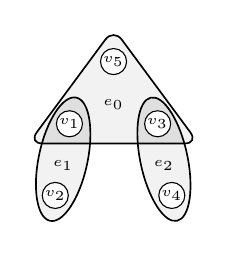
\begin{tikzpicture}[
    scale=1.0,
    every node/.style={transform shape},
    vertex/.style={
        circle, draw, fill=white, font=\tiny,
        minimum size=0.33cm, inner sep=0.4pt
    },
    hfill/.style={
        draw=none, fill=gray!22, fill opacity=0.45
    },
    hint/.style={
        draw=none, fill=gray!50, fill opacity=0.28
    },
    hborder/.style={
        draw, line width=0.6pt, fill=none
    },
    elabel/.style={font=\tiny}
]

  % ============================================================
  % Light fills
  % ============================================================

  % e1
  \fill[hfill, rounded corners=5pt]
      ( 0.00,  0.22)
   -- (-1.08, -1.24)
   -- ( 1.08, -1.24)
   -- cycle;

  % e2
  \fill[hfill, rotate around={-12:(-0.64,-1.44)}]
      (-0.64,-1.44) ellipse [x radius=0.31, y radius=0.80];

  % e3
  \fill[hfill, rotate around={12:(0.64,-1.44)}]
      (0.64,-1.44) ellipse [x radius=0.30, y radius=0.80];

  % ============================================================
  % Explicit darker intersections
  % ============================================================

  % e1 ∩ e2
  \begin{scope}
    \clip[rounded corners=5pt]
        ( 0.00,  0.22)
     -- (-1.08, -1.24)
     -- ( 1.08, -1.24)
     -- cycle;
    \fill[hint, rotate around={-12:(-0.64,-1.44)}]
        (-0.64,-1.44) ellipse [x radius=0.31, y radius=0.80];
  \end{scope}

  % e1 ∩ e3
  \begin{scope}
    \clip[rounded corners=5pt]
        ( 0.00,  0.22)
     -- (-1.08, -1.24)
     -- ( 1.08, -1.24)
     -- cycle;
    \fill[hint, rotate around={12:(0.64,-1.44)}]
        (0.64,-1.44) ellipse [x radius=0.30, y radius=0.80];
  \end{scope}

  % ============================================================
  % Borders
  % ============================================================

  % e1
  \draw[hborder, rounded corners=5pt]
      ( 0.00,  0.22)
   -- (-1.08, -1.24)
   -- ( 1.08, -1.24)
   -- cycle;

  % e2
  \draw[hborder, rotate around={-12:(-0.64,-1.44)}]
      (-0.64,-1.44) ellipse [x radius=0.31, y radius=0.80];

  % e3
  \draw[hborder, rotate around={12:(0.64,-1.44)}]
      (0.64,-1.44) ellipse [x radius=0.30, y radius=0.80];

  % Labels
  \node[elabel] at ( 0.00,-0.75) {$e_0$};
  \node[elabel] at (-0.64,-1.52) {$e_1$};
  \node[elabel] at ( 0.64,-1.52) {$e_2$};

  % Vertices last
  \node[vertex] (v5) at ( 0.00, -0.20) {$v_5$};
  \node[vertex] (v1) at (-0.56, -0.99) {$v_1$};
  \node[vertex] (v3) at ( 0.56, -0.99) {$v_3$};
  \node[vertex] (v2) at (-0.74, -1.90) {$v_2$};
  \node[vertex] (v4) at ( 0.74, -1.90) {$v_4$};

\end{tikzpicture}}\\
        \resizebox{\linewidth}{!}{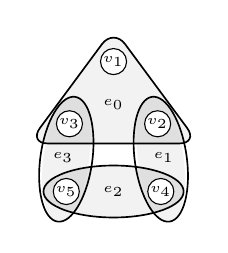
\begin{tikzpicture}[
    scale=1.0,
    every node/.style={transform shape},
    vertex/.style={
        circle, draw, fill=white, font=\tiny,
        minimum size=0.33cm, inner sep=0.4pt
    },
    hfill/.style={
        draw=none, fill=gray!22, fill opacity=0.45
    },
    hint/.style={
        draw=none, fill=gray!50, fill opacity=0.28
    },
    hborder/.style={
        draw, line width=0.6pt, fill=none
    },
    elabel/.style={font=\tiny}
]

  % ============================================================
  % Light fills
  % ============================================================

  % e1
  \fill[hfill, rounded corners=7pt]
      ( 0.00,  0.22)
   -- (-1.08, -1.24)
   -- ( 1.08, -1.24)
   -- cycle;

  % e4
  \fill[hfill, rotate around={-8:(-0.6,-1.44)}]
      (-0.6,-1.44) ellipse [x radius=0.29, y radius=0.80];

  % e2
  \fill[hfill, rotate around={8:(0.6,-1.44)}]
      (0.6,-1.44) ellipse [x radius=0.29, y radius=0.80];

  % e3
  \fill[hfill]
      (0.00,-1.85) ellipse [x radius=0.89, y radius=0.33];


  % ============================================================
  % Explicit darker intersections
  % ============================================================

  % e1 ∩ e4
  \begin{scope}
    \clip[rounded corners=7pt]
        ( 0.00,  0.22)
     -- (-1.08, -1.24)
     -- ( 1.08, -1.24)
     -- cycle;
    \fill[hint, rotate around={-8:(-0.6,-1.44)}]
        (-0.6,-1.44) ellipse [x radius=0.33, y radius=0.80];
  \end{scope}

  % e1 ∩ e2
  \begin{scope}
    \clip[rounded corners=7pt]
        ( 0.00,  0.22)
     -- (-1.08, -1.24)
     -- ( 1.08, -1.24)
     -- cycle;
    \fill[hint, rotate around={8:(0.6,-1.44)}]
        (0.6,-1.44) ellipse [x radius=0.33, y radius=0.80];
  \end{scope}

  % e3 ∩ e4
  \begin{scope}
    \clip (0.00,-1.85) ellipse [x radius=0.89, y radius=0.33];
    \fill[hint, rotate around={-8:(-0.6,-1.44)}]
        (-0.6,-1.44) ellipse [x radius=0.33, y radius=0.80];
  \end{scope}

  % e3 ∩ e2
  \begin{scope}
    \clip (0.00,-1.85) ellipse [x radius=0.89, y radius=0.33];
    \fill[hint, rotate around={8:(0.6,-1.44)}]
        (0.6,-1.44) ellipse [x radius=0.33, y radius=0.80];
  \end{scope}


  % ============================================================
  % Borders
  % ============================================================

  % e1
  \draw[hborder, rounded corners=7pt]
      ( 0.00,  0.22)
   -- (-1.08, -1.24)
   -- ( 1.08, -1.24)
   -- cycle;

  % e4
  \draw[hborder, rotate around={-8:(-0.6,-1.44)}]
      (-0.6,-1.44) ellipse [x radius=0.33, y radius=0.80];

  % e2
  \draw[hborder, rotate around={8:(0.6,-1.44)}]
      (0.6,-1.44) ellipse [x radius=0.33, y radius=0.80];

  % e3
  \draw[hborder]
      (0.00,-1.85) ellipse [x radius=0.89, y radius=0.33];


  % Labels
  \node[elabel] at ( 0.00,-0.75) {$e_0$};
  \node[elabel] at (-0.64,-1.42) {$e_3$};
  \node[elabel] at ( 0.64,-1.42) {$e_1$};
  \node[elabel] at ( 0.00,-1.85) {$e_2$};

  % Vertices last
  \node[vertex] (v1) at ( 0.00, -0.20) {$v_1$};
  \node[vertex] (v3) at (-0.56, -0.99) {$v_3$};
  \node[vertex] (v2) at ( 0.56, -0.99) {$v_2$};
  \node[vertex] (v5) at (-0.60, -1.85) {$v_5$};
  \node[vertex] (v4) at ( 0.60, -1.85) {$v_4$};

\end{tikzpicture}}\\
        [2pt]
        {\small (a) Hypergraphs}
    \end{minipage}\hfill
    \begin{minipage}[b]{0.30\linewidth}\centering
        \resizebox{\linewidth}{!}{% Auto-generated compact DD for FLOWER (order ['v1', 'v0', 'v3', 'v4', 'v2'], width 3)
% x-coordinates widened (x1.5) to avoid node overlap; y-coordinates (height) unchanged.
\begin{tikzpicture}[
    >=Stealth, thick,
    sn/.style={ellipse, draw, fill=gray!12, font=\tiny, inner sep=0.8pt, minimum width=0.85cm, minimum height=0.38cm},
    za/.style={draw, dashed, gray, ->, line width=0.4pt},
    oa/.style={draw, ->, line width=0.5pt}]
  \node[sn] (n0) at (0.00,0.00) {$\emptyset$};
  \node[sn] (n1) at (-0.74,-0.92) {$\emptyset$};
  \node[sn] (n2) at (0.74,-0.92) {$\{e_0,e_1\}$};
  \node[sn] (n3) at (-0.74,-1.84) {$\emptyset$};
  \node[sn] (n4) at (0.74,-1.84) {$\{e_0\}$};
  \node[sn] (n5) at (-1.47,-2.76) {$\emptyset$};
  \node[sn] (n6) at (0.00,-2.76) {$\{e_2\}$};
  \node[sn] (n7) at (1.47,-2.76) {$\{e_0,e_2\}$};
  \node[sn] (n8) at (-0.74,-3.68) {$\emptyset$};
  \node[sn] (n9) at (0.74,-3.68) {$\{e_0\}$};
  \node[sn] (n10) at (0.00,-4.60) {$\emptyset$};
  \draw[za] (n0) to (n1);
  \draw[oa] (n0) to (n2);
  \draw[za, bend right=16] (n1) to (n3);
  \draw[oa, bend left=16] (n1) to (n3);
  \draw[za, bend right=16] (n2) to (n4);
  \draw[oa, bend left=16] (n2) to (n4);
  \draw[za] (n3) to (n5);
  \draw[oa] (n3) to (n6);
  \draw[za] (n4) to (n5);
  \draw[oa] (n4) to (n7);
  \draw[za, bend right=16] (n5) to (n8);
  \draw[oa, bend left=16] (n5) to (n8);
  \draw[za, bend right=16] (n7) to (n9);
  \draw[oa, bend left=16] (n7) to (n9);
  \draw[za, bend right=16] (n6) to (n8);
  \draw[oa, bend left=16] (n6) to (n8);
  \draw[za, bend right=16] (n8) to (n10);
  \draw[oa, bend left=16] (n8) to (n10);
  \draw[za, bend right=16] (n9) to (n10);
  \draw[oa, bend left=16] (n9) to (n10);
\end{tikzpicture}
}\\[3pt]
        {\small (b) Flower DD}
    \end{minipage}\hfill
    \begin{minipage}[b]{0.40\linewidth}\centering
        \resizebox{\linewidth}{!}{% Auto-generated compact DD for CYCLE (order ['v2', 'v3', 'v4', 'v1', 'v0'], width 4)
% x-coordinates widened (x1.5) to avoid node overlap; y-coordinates (height) unchanged.
\begin{tikzpicture}[
    >=Stealth, thick,
    sn/.style={ellipse, draw, fill=gray!12, font=\tiny, inner sep=0.8pt, minimum width=0.85cm, minimum height=0.38cm},
    za/.style={draw, dashed, gray, ->, line width=0.4pt},
    oa/.style={draw, ->, line width=0.5pt}]
  \node[sn] (n0) at (0.00,0.00) {$\emptyset$};
  \node[sn] (n1) at (-0.74,-0.92) {$\emptyset$};
  \node[sn] (n2) at (0.74,-0.92) {$\{e_0\}$};
  \node[sn] (n3) at (-1.47,-1.84) {$\emptyset$};
  \node[sn] (n4) at (0.00,-1.84) {$\{e_1\}$};
  \node[sn] (n5) at (1.47,-1.84) {$\{e_0,e_1\}$};
  \node[sn] (n6) at (-2.21,-2.76) {$\emptyset$};
  \node[sn] (n7) at (-0.74,-2.76) {$\{e_3\}$};
  \node[sn] (n8) at (0.74,-2.76) {$\{e_1\}$};
  \node[sn] (n9) at (2.21,-2.76) {$\{e_1,e_3\}$};
  \node[sn] (n10) at (-2.21,-3.68) {$\emptyset$};
  \node[sn] (n11) at (-0.74,-3.68) {$\{e_2\}$};
  \node[sn] (n12) at (0.74,-3.68) {$\{e_3\}$};
  \node[sn] (n13) at (2.21,-3.68) {$\{e_2,e_3\}$};
  \node[sn] (n14) at (0.00,-4.60) {$\emptyset$};
  \draw[za] (n0) to (n1);
  \draw[oa] (n0) to (n2);
  \draw[za] (n1) to (n3);
  \draw[oa] (n1) to (n4);
  \draw[za] (n2) to (n3);
  \draw[oa] (n2) to (n5);
  \draw[za] (n3) to (n6);
  \draw[oa] (n3) to (n7);
  \draw[za] (n4) to (n8);
  \draw[oa] (n4) to (n9);
  \draw[za] (n5) to (n8);
  \draw[oa] (n5) to (n9);
  \draw[za] (n6) to (n10);
  \draw[oa] (n6) to (n11);
  \draw[za] (n8) to (n10);
  \draw[oa] (n8) to (n11);
  \draw[za] (n7) to (n12);
  \draw[oa] (n7) to (n13);
  \draw[za] (n9) to (n12);
  \draw[oa] (n9) to (n13);
  \draw[za, bend right=16] (n10) to (n14);
  \draw[oa, bend left=16] (n10) to (n14);
  \draw[za, bend right=16] (n13) to (n14);
  \draw[oa, bend left=16] (n13) to (n14);
  \draw[za, bend right=16] (n11) to (n14);
  \draw[oa, bend left=16] (n11) to (n14);
  \draw[za, bend right=16] (n12) to (n14);
  \draw[oa, bend left=16] (n12) to (n14);
\end{tikzpicture}
}\\[3pt]
        {\small (c) Cycle DD}
    \end{minipage}
    \caption{Bounded-width compact DDs for a flower and a cycle hypergraph, described in
    Example~\ref{exa:bounded-compact-dds}: (a) the flower and cycle hypergraphs, (b) the
    flower DD of width $3$, and (c) the cycle DD of width $4$.}
    \label{fig:dd-structures}
\end{figure}

% \begin{figure}
%     \centering
%     \includegraphics[width=0.5\linewidth]{Figures/placeholders/Flower visualization placeholder.png}
%     \caption{Flower structure placeholder.}
%     \label{fig:placeholder}
% \end{figure}

% \begin{figure}
%     \centering
%     \includegraphics[width=0.5\linewidth]{Figures/placeholders/Flower BDD placeholder.png}
%     \caption{DD for flower of figure. Black denotes 1-arcs, grey 0-arcs.}
%     \label{fig:placeholder}
% \end{figure}

% \begin{figure}
%     \centering
%     \includegraphics[width=0.5\linewidth]{Figures/placeholders/Cyclic hypergraph placeholder.png}
%     \caption{Cyclic structure placeholder.}
%     \label{fig:placeholder}
% \end{figure}

% \begin{figure}
%     \centering
%     \includegraphics[width=0.5\linewidth]{Figures/placeholders/BDD placeholder for cycle.png}
%     \caption{DD for cycle of figure. Black denotes 1-arcs, grey 0-arcs.}
%     \label{fig:placeholder}
% \end{figure}

\subsection{Valid antichains, pathwidth,  and incidence treewidth}
\label{subsec:vaw_treewidth_relation}

Researchers have also characterized the hypergraph through \emph{incidence treewidth} to build polynomial-size extended formulations for BPO using a d-DNNF representation~\cite{capelliDelPiaDiGregorio2024kc}. We now show that the valid antichains characterized here are indeed incomparable with the incidence treewidth in Proposition \ref{prop:va-vs-treewidth}. Recall that treewidth is the minimum, over all tree decompositions, of the largest bag size minus one~\cite{diestel2017graph}. The incidence treewidth of a hypergraph is the treewidth of its incidence graph.

Before proving the incomparability, we recall that for ordinary graphs (i.e., rank-two hypergraphs) the valid-antichain width is governed exactly by a classical width parameter. For a graph $G=(V,E)$ and an order $\sigma=(v_1,\ldots,v_n)$ with prefixes $U_i=\{v_1,\ldots,v_i\}$, let $b_i(\sigma)=\left|\{v\in U_i : \exists\, w\in V\setminus U_i \text{ with } \{v,w\}\in E\}\right|$ be the number of \emph{boundary} vertices at $U_i$. The \emph{vertex separation} of $\sigma$ is $\operatorname{vs}_\sigma(G)=\max_{i\in\{1,\ldots,n\}} b_i(\sigma)$, and the \emph{vertex separation number} is $\operatorname{vs}(G)=\min_\sigma \operatorname{vs}_\sigma(G)$. By a classical result, the vertex separation number coincides with pathwidth (i.e., a number that shows how close a graph is to being a path), that is, $\operatorname{vs}(G)=\operatorname{pw}(G)$~\cite{kinnersley1992pathwidth}.

\begin{corollary}\label{cor:vaw-pathwidth}
For every ordinary graph $G=(V,E)$, $\operatorname{VAW}(G)=2^{\operatorname{vs}(G)}=2^{\operatorname{pw}(G)}$.
\end{corollary}

\begin{proof}
Fix an order $\sigma$. At any prefix $U_i$, each active edge has exactly one endpoint in $U_i$ and one outside, so every reduced active edge is a singleton $\{v\}$ with $v$ a boundary vertex, and these singletons are pairwise incomparable. Hence every subset of the $b_i(\sigma)$ boundary singletons is a valid antichain, giving $|\operatorname{VA}_i(\sigma)|=2^{b_i(\sigma)}$. Since $x\mapsto 2^x$ is increasing, $W(\sigma)=\max_i 2^{b_i(\sigma)}=2^{\operatorname{vs}_\sigma(G)}$, and minimizing over $\sigma$ yields $\operatorname{VAW}(G)=2^{\operatorname{vs}(G)}$. The identity $\operatorname{vs}(G)=\operatorname{pw}(G)$~\cite{kinnersley1992pathwidth} gives the last equality. \hfill$\square$
\end{proof}

We note that this identity is specific to rank-two hypergraphs; for hypergraphs of higher rank, valid-antichain width departs from pathwidth, as the converse direction below shows.


\begin{proposition} \label{prop:va-vs-treewidth}
The valid antichain characterization is incomparable to the incidence treewidth.
\end{proposition}

\begin{proof}
We first show that bounded incidence treewidth does not imply bounded VAW. Consider $T_h=(V,E)$, the complete binary tree of height $h$, where each edge has exactly two vertices. Since $T_h$ is a tree, its treewidth is one. Moreover, the incidence graph of $T_h$ is obtained by subdividing every edge of $T_h$ once, so each original edge becomes an incidence node adjacent to its two endpoints; the incidence graph is therefore also a tree and has treewidth one. On the other hand, complete binary trees have unbounded pathwidth as $h$ grows~\cite{diestel2017graph}. Hence, by Corollary~\ref{cor:vaw-pathwidth}, $\operatorname{VAW}(T_h)=2^{\operatorname{pw}(T_h)}$ is also unbounded. Thus, the family $\{T_h\}_{h\ge 1}$ has bounded incidence treewidth but unbounded VAW.

We now show the converse also fails. Let $A=\{a_1,\ldots,a_p\}$ and
$B=\{b_1,\ldots,b_q\}$ be sets of vertices, and define a hypergraph $G=(V,E)$ with $V=A\cup B$, and $E=\{A\cup\{b\}: b\in B\}$. Order all vertices of $A$ first and then all vertices of $B$. At any prefix $U_i$ of this order, all active hyperedges have the same reduced active hyperedge. Therefore, there are at most two valid antichains, the empty one and the singleton containing that common
reduced hyperedge, so $|\operatorname{VA}_i(\sigma)| \le 2$. On the other hand, the incidence graph contains a complete bipartite graph between $A$ and the hyperedges, so its incidence treewidth is unbounded as the number of vertices grows.\hfill$\square$
\end{proof}

% \subsection{Worst-case size}
% \label{subsec:compact_bdd_worst_case}

% The complete hypergraph shows that exponential worst-case size is unavoidable. Let
% $K_n^{\mathrm{full}}$ be the hypergraph on $n$ vertices containing every hyperedge of
% cardinality at least two. For any order and any layer $i<n$, every nonempty subset of
% $U_i$ appears as a reduced active hyperedge: if $R\subseteq U_i$ is nonempty, then
% $R\cup\{v\}$ is a hyperedge for any unassigned vertex $v$.

% The valid antichains at layer $i$ are exactly
% \[
% \emptyset
% \quad\text{and}\quad
% \{R\}\ \text{ for each nonempty } R\subseteq U_i.
% \]
% Indeed, if a valid antichain has union $X$, then $X$ itself is a reduced active
% hyperedge and must be contained in one of the antichain members, forcing that member to
% equal $X$. Therefore
% \[
% |\operatorname{VA}_i(\sigma)|
% =
% 1+(2^{|U_i|}-1)
% =
% 2^{|U_i|}.
% \]
% The maximum width is $2^{n-1}$, and the number of internal nonterminal nodes is
% \[
% \sum_{i=0}^{n-1} 2^i = 2^n-1.
% \]
% Thus the compact construction does not avoid the exponential worst case in general.

